\chapter{Birkhoff–-vonNeumannの定理}
\label{vonNeumann}

\chapter{人工データに対する予測結果}
\label{chap:artificial}

\ref{chap:ex}章で掲載した人工データに対する実験結果の他にも,4行,8行毎に各周波数成分をシャッフルした場合の実験も行った.
以下に実験結果を掲載する.

%%%%%%%%%%%%%%%%%%%%%%%%%%%%
\begin{figure*}[!t]
    \centering
    \subfloat[Percentage of correct answers for training and validation data.]{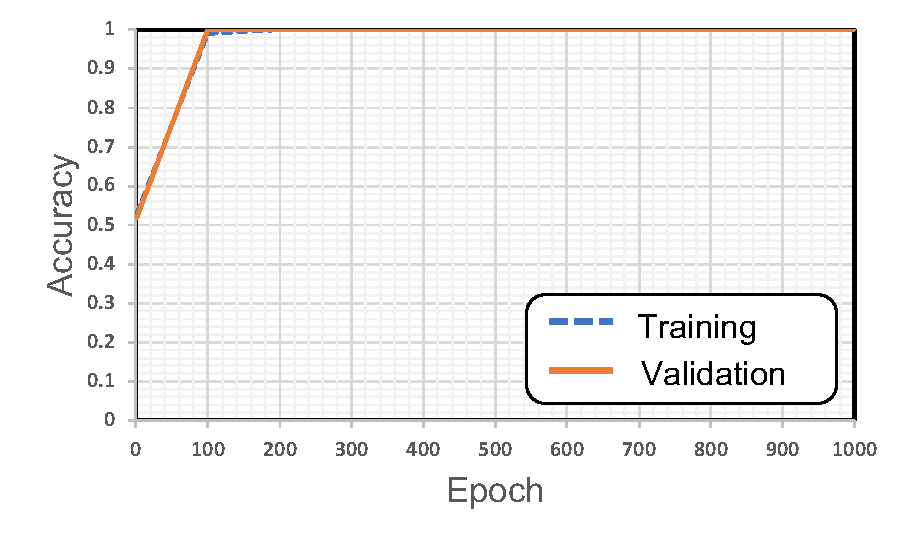
\includegraphics[clip, width=4.5in]{figures/graph/01mat_4block.pdf}
    \label{fig:acc_01mat_4block}}
    \\
    \subfloat[Spectrogram of estimated signal and predictive separation signal.]{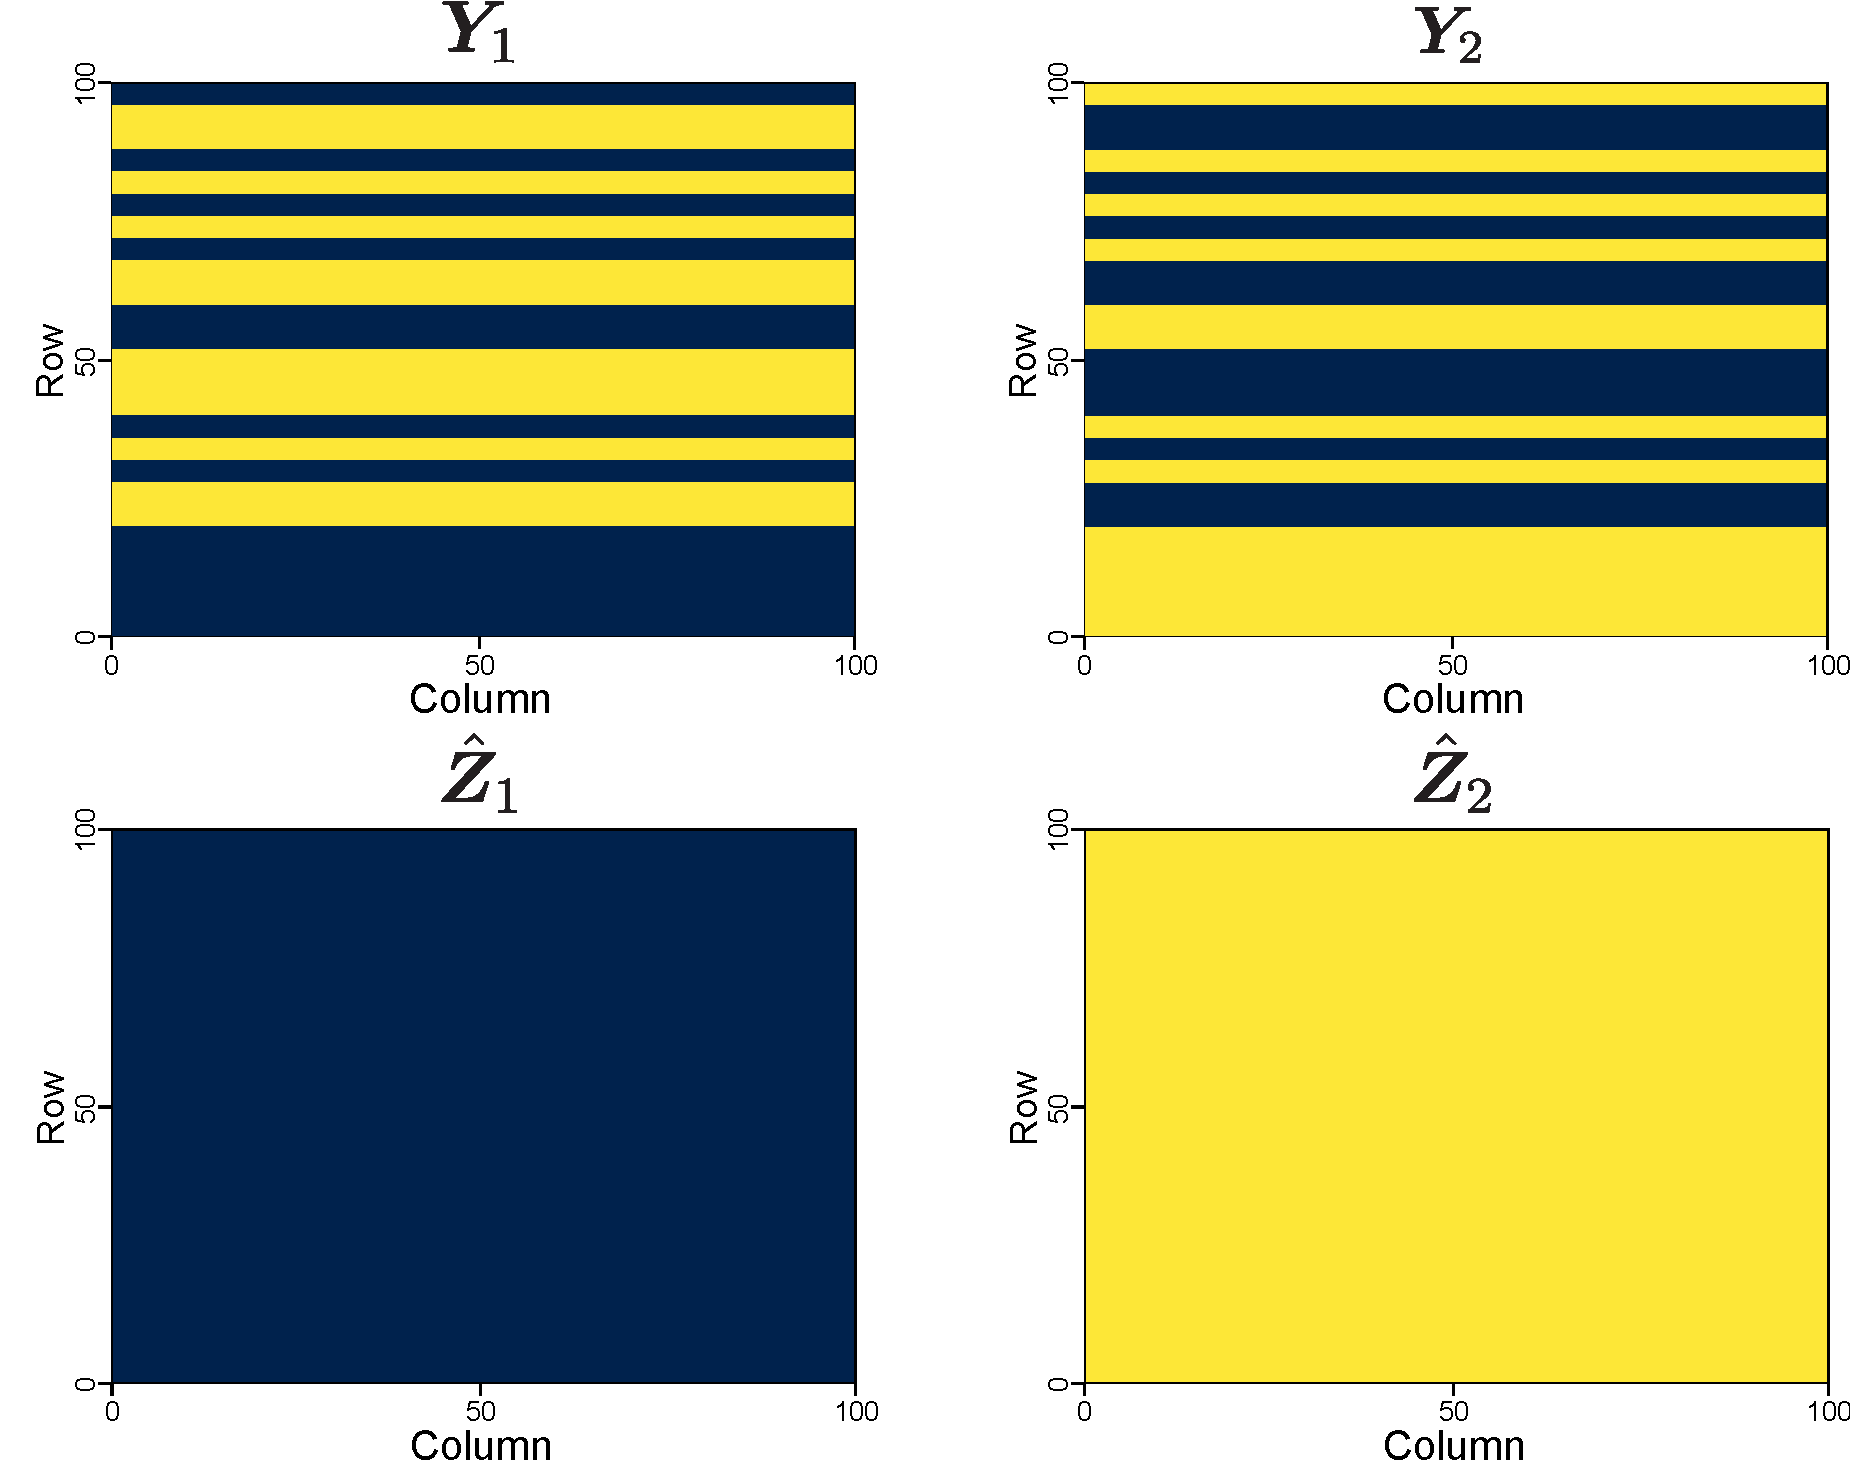
\includegraphics[clip, width=5.0in]{figures/01mat_4block.pdf}
    \label{fig:spec_01mat_4block}}  
    \caption{Experimental results using matrix of Fig~\ref{fig:01mat_spec} (randomly shuffle every four rows).}
    \label{fig:01mat_4block}
\end{figure*}
%%%%%%%%%%%%%%%%%%%%%%%%%%%%

%%%%%%%%%%%%%%%%%%%%%%%%%%%%
\begin{figure*}[!t]
    \centering
    \subfloat[Percentage of correct answers for training and validation data.]{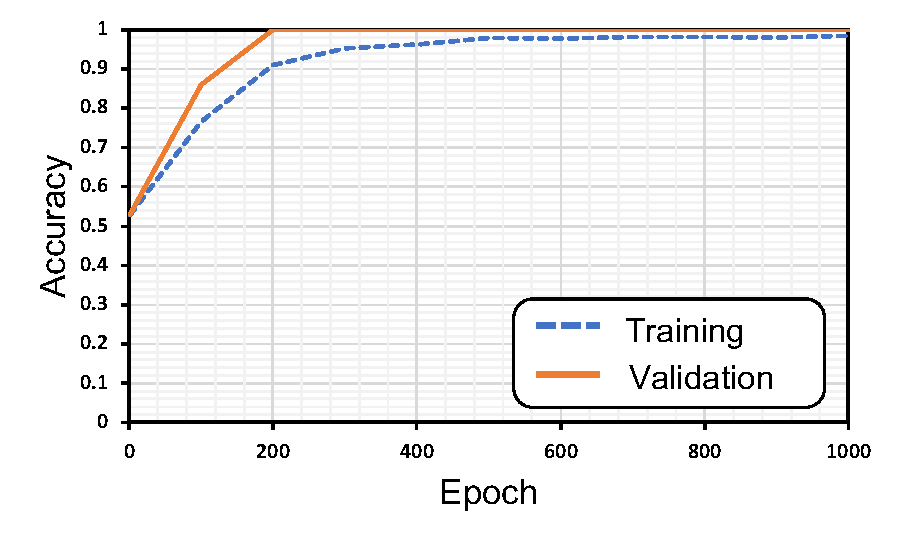
\includegraphics[clip, width=4.5in]{figures/graph/25stripe_4block.pdf}
    \label{fig:acc_25mat_4block}}
    \\
    \subfloat[Spectrogram of estimated signal and predictive separation signal.]{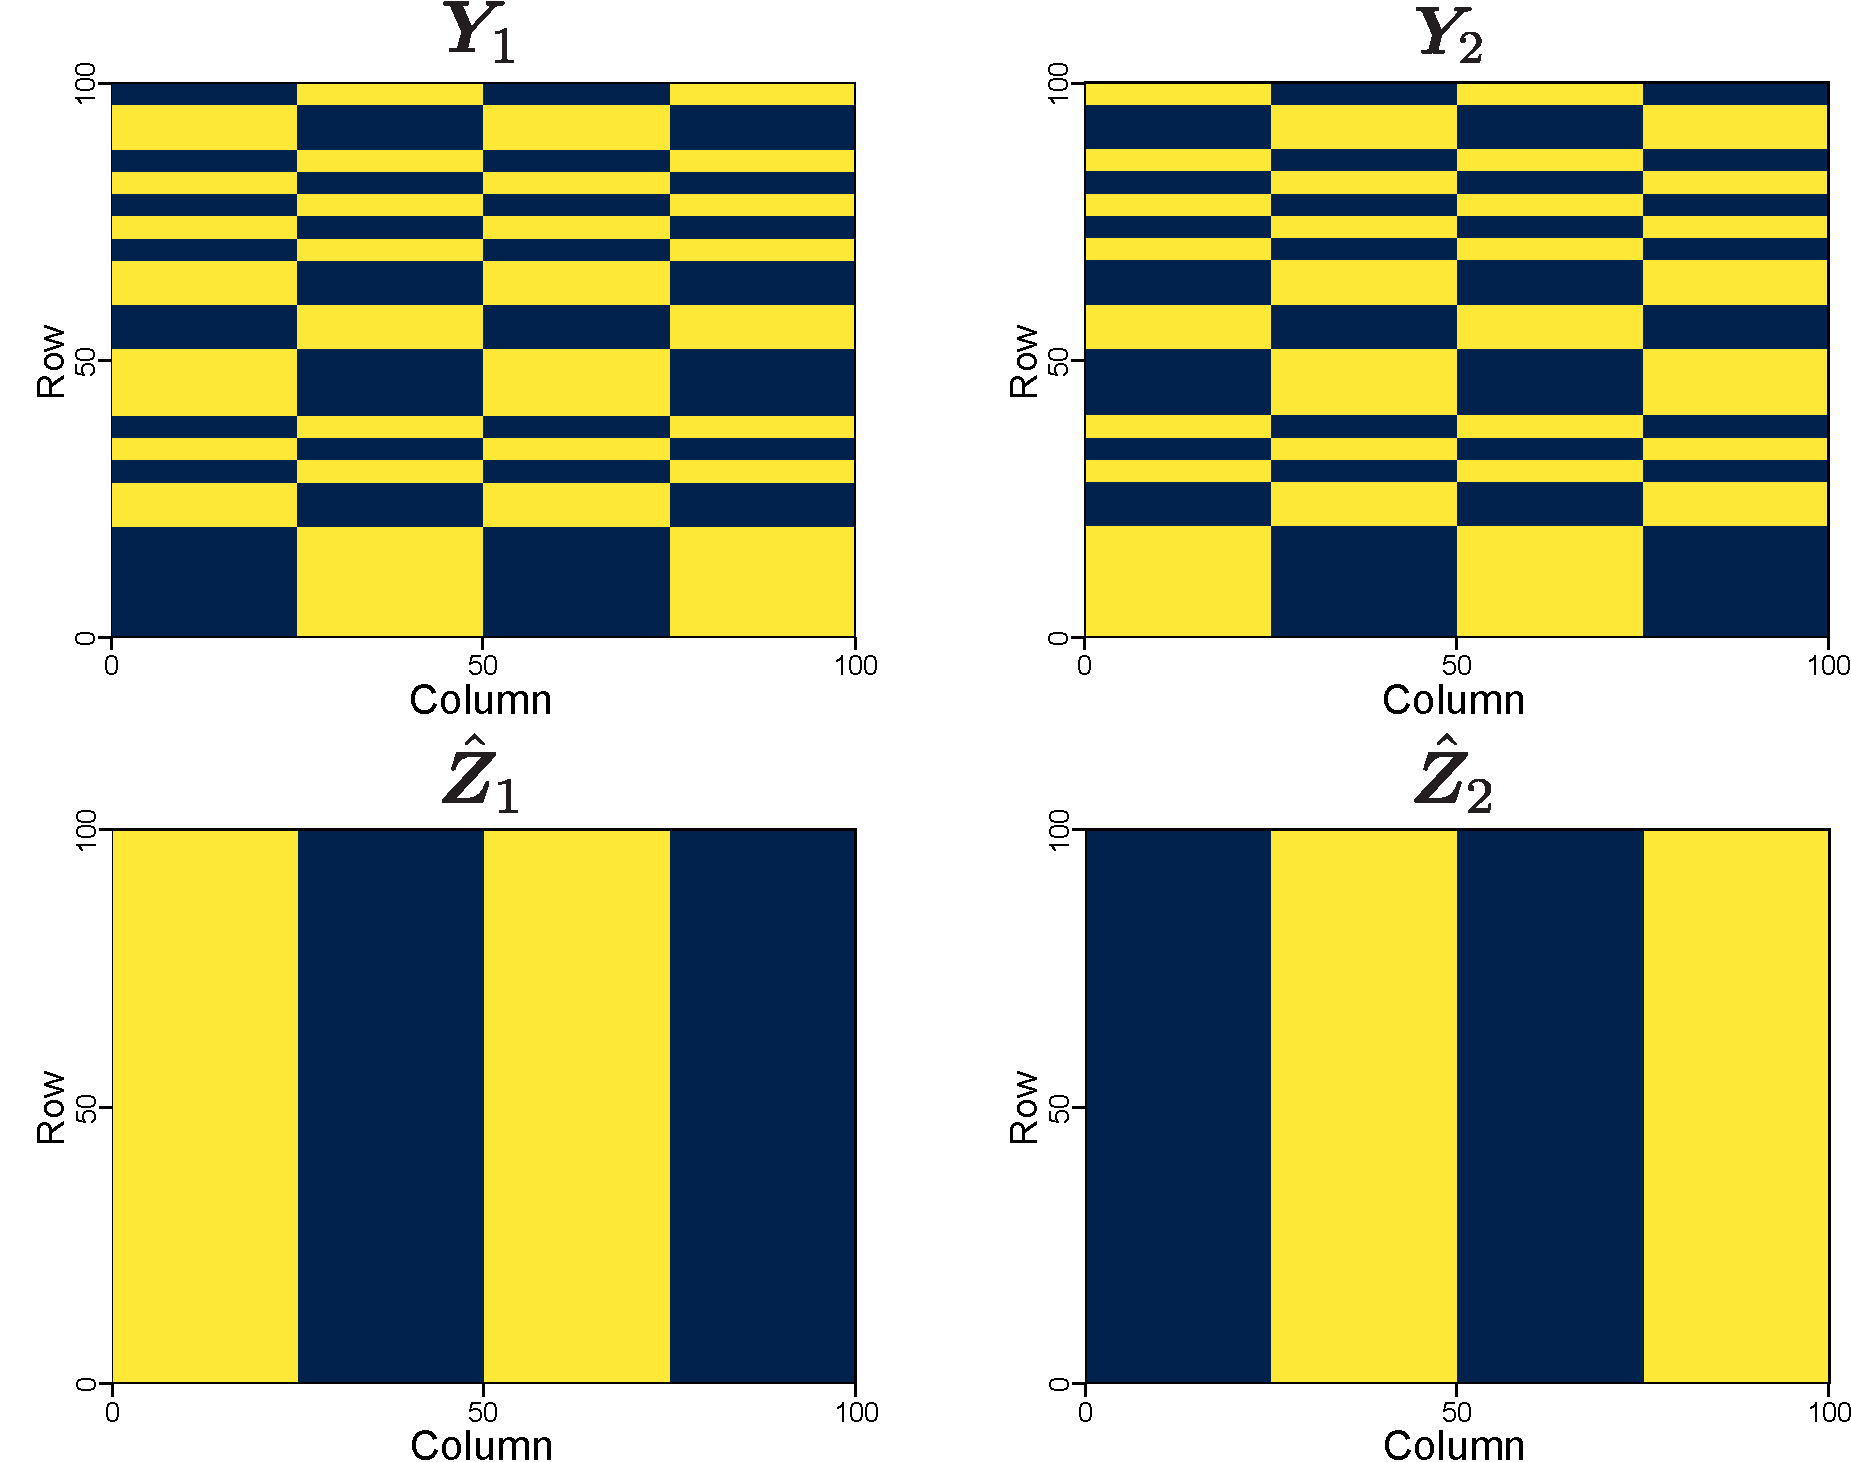
\includegraphics[clip, width=5.0in]{figures/25stripe_4block.pdf}
    \label{fig:spec_25mat_4block}}  
    \caption{Experimental results using the matrix of Fig~\ref{fig:25stripe_spec} (randomly shuffle four rows).}
    \label{fig:25mat_4block}
\end{figure*}
%%%%%%%%%%%%%%%%%%%%%%%%%%%%

%%%%%%%%%%%%%%%%%%%%%%%%%%%%
\begin{figure*}[!t]
    \centering
    \subfloat[Percentage of correct answers for training and validation data.]{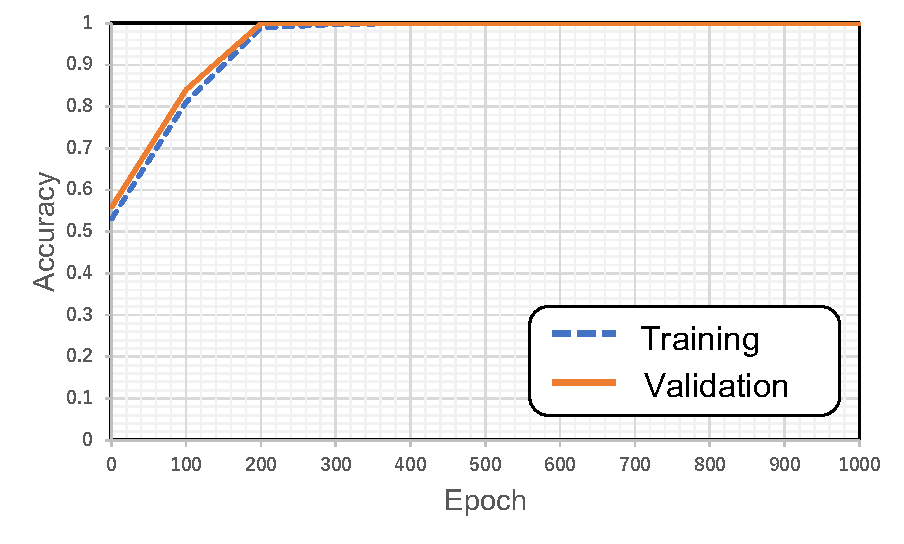
\includegraphics[clip, width=4.5in]{figures/graph/stripe_4block.pdf}
    \label{fig:acc_stripe_4block}}
    \\
    \subfloat[Spectrogram of estimated signal and predictive separation signal.]{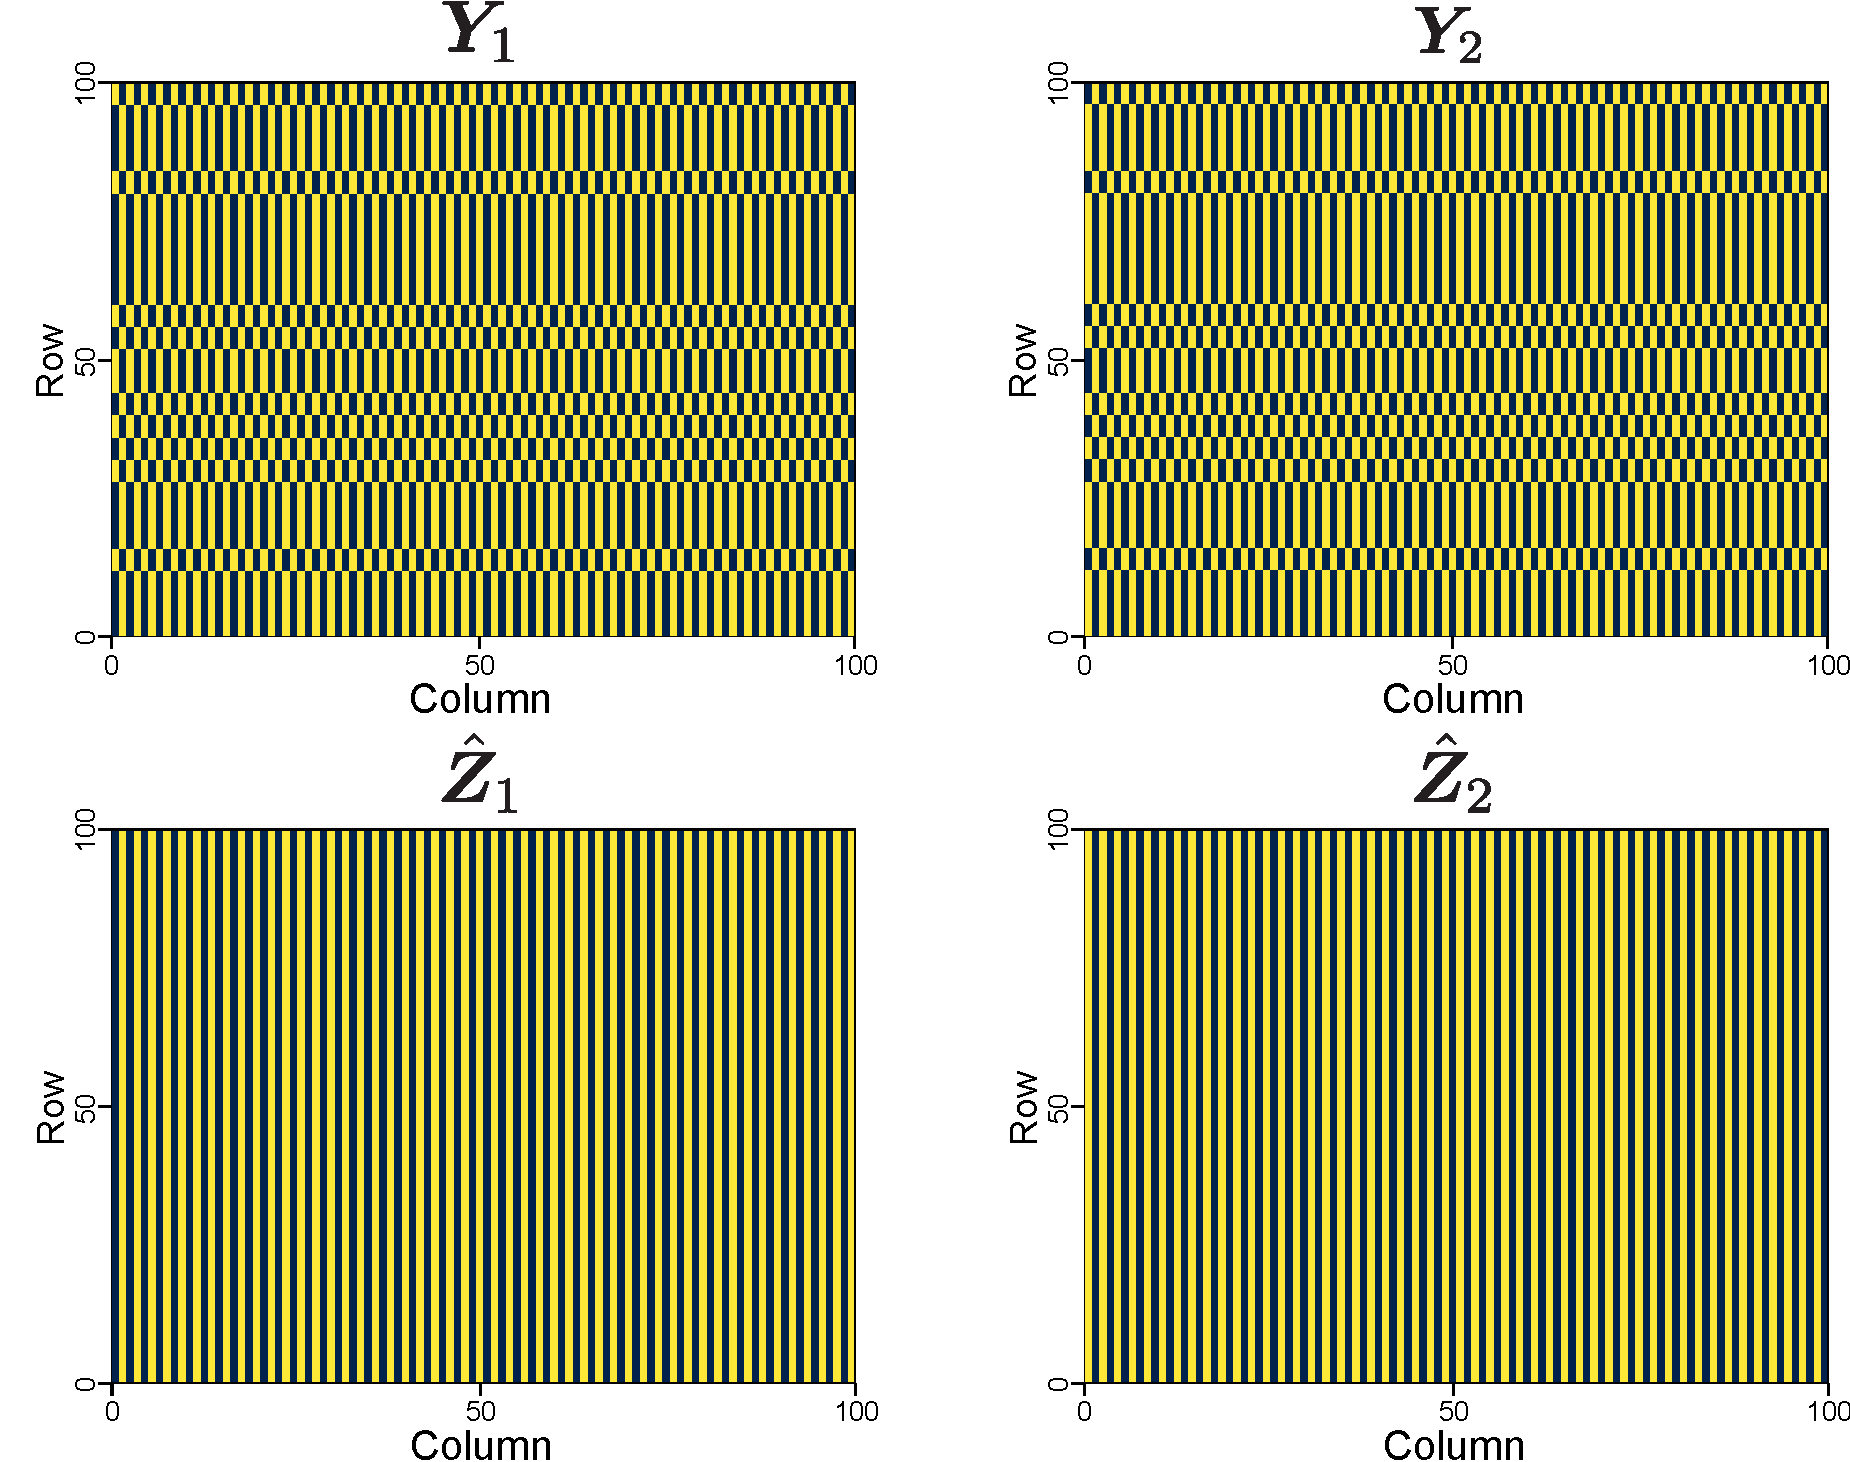
\includegraphics[clip, width=5.0in]{figures/stripe_4block.pdf}
    \label{fig:spec_stripe_4block}}  
    \caption{Experimental results using the matrix of Fig~\ref{fig:stripe_spec} (randomly shuffle four rows).}
    \label{fig:stripe_4block}
\end{figure*}
%%%%%%%%%%%%%%%%%%%%%%%%%%%%

%%%%%%%%%%%%%%%%%%%%%%%%%%%%
\begin{figure*}[!t]
    \centering
    \subfloat[Percentage of correct answers for training and validation data.]{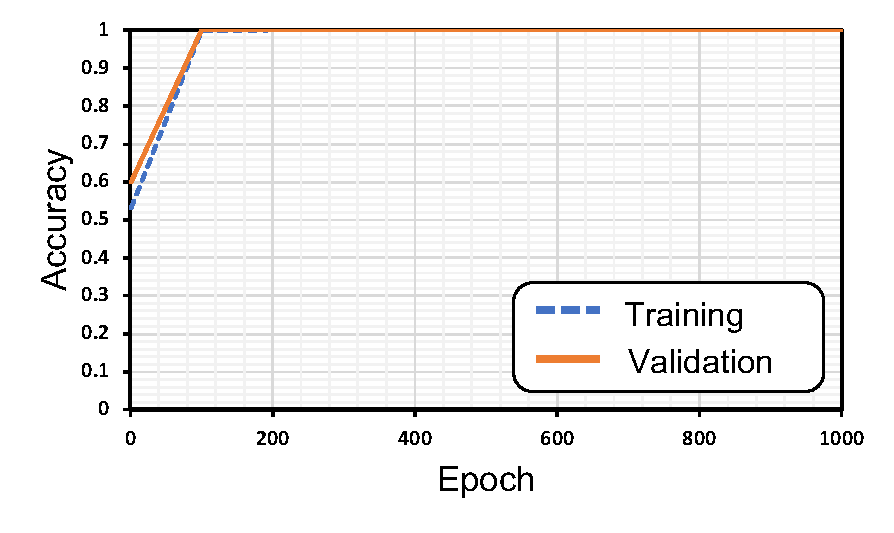
\includegraphics[clip, width=4.5in]{figures/graph/01mat_8block.pdf}
    \label{fig:acc_01mat_8block}}
    \\
    \subfloat[Spectrogram of estimated signal and predictive separation signal.]{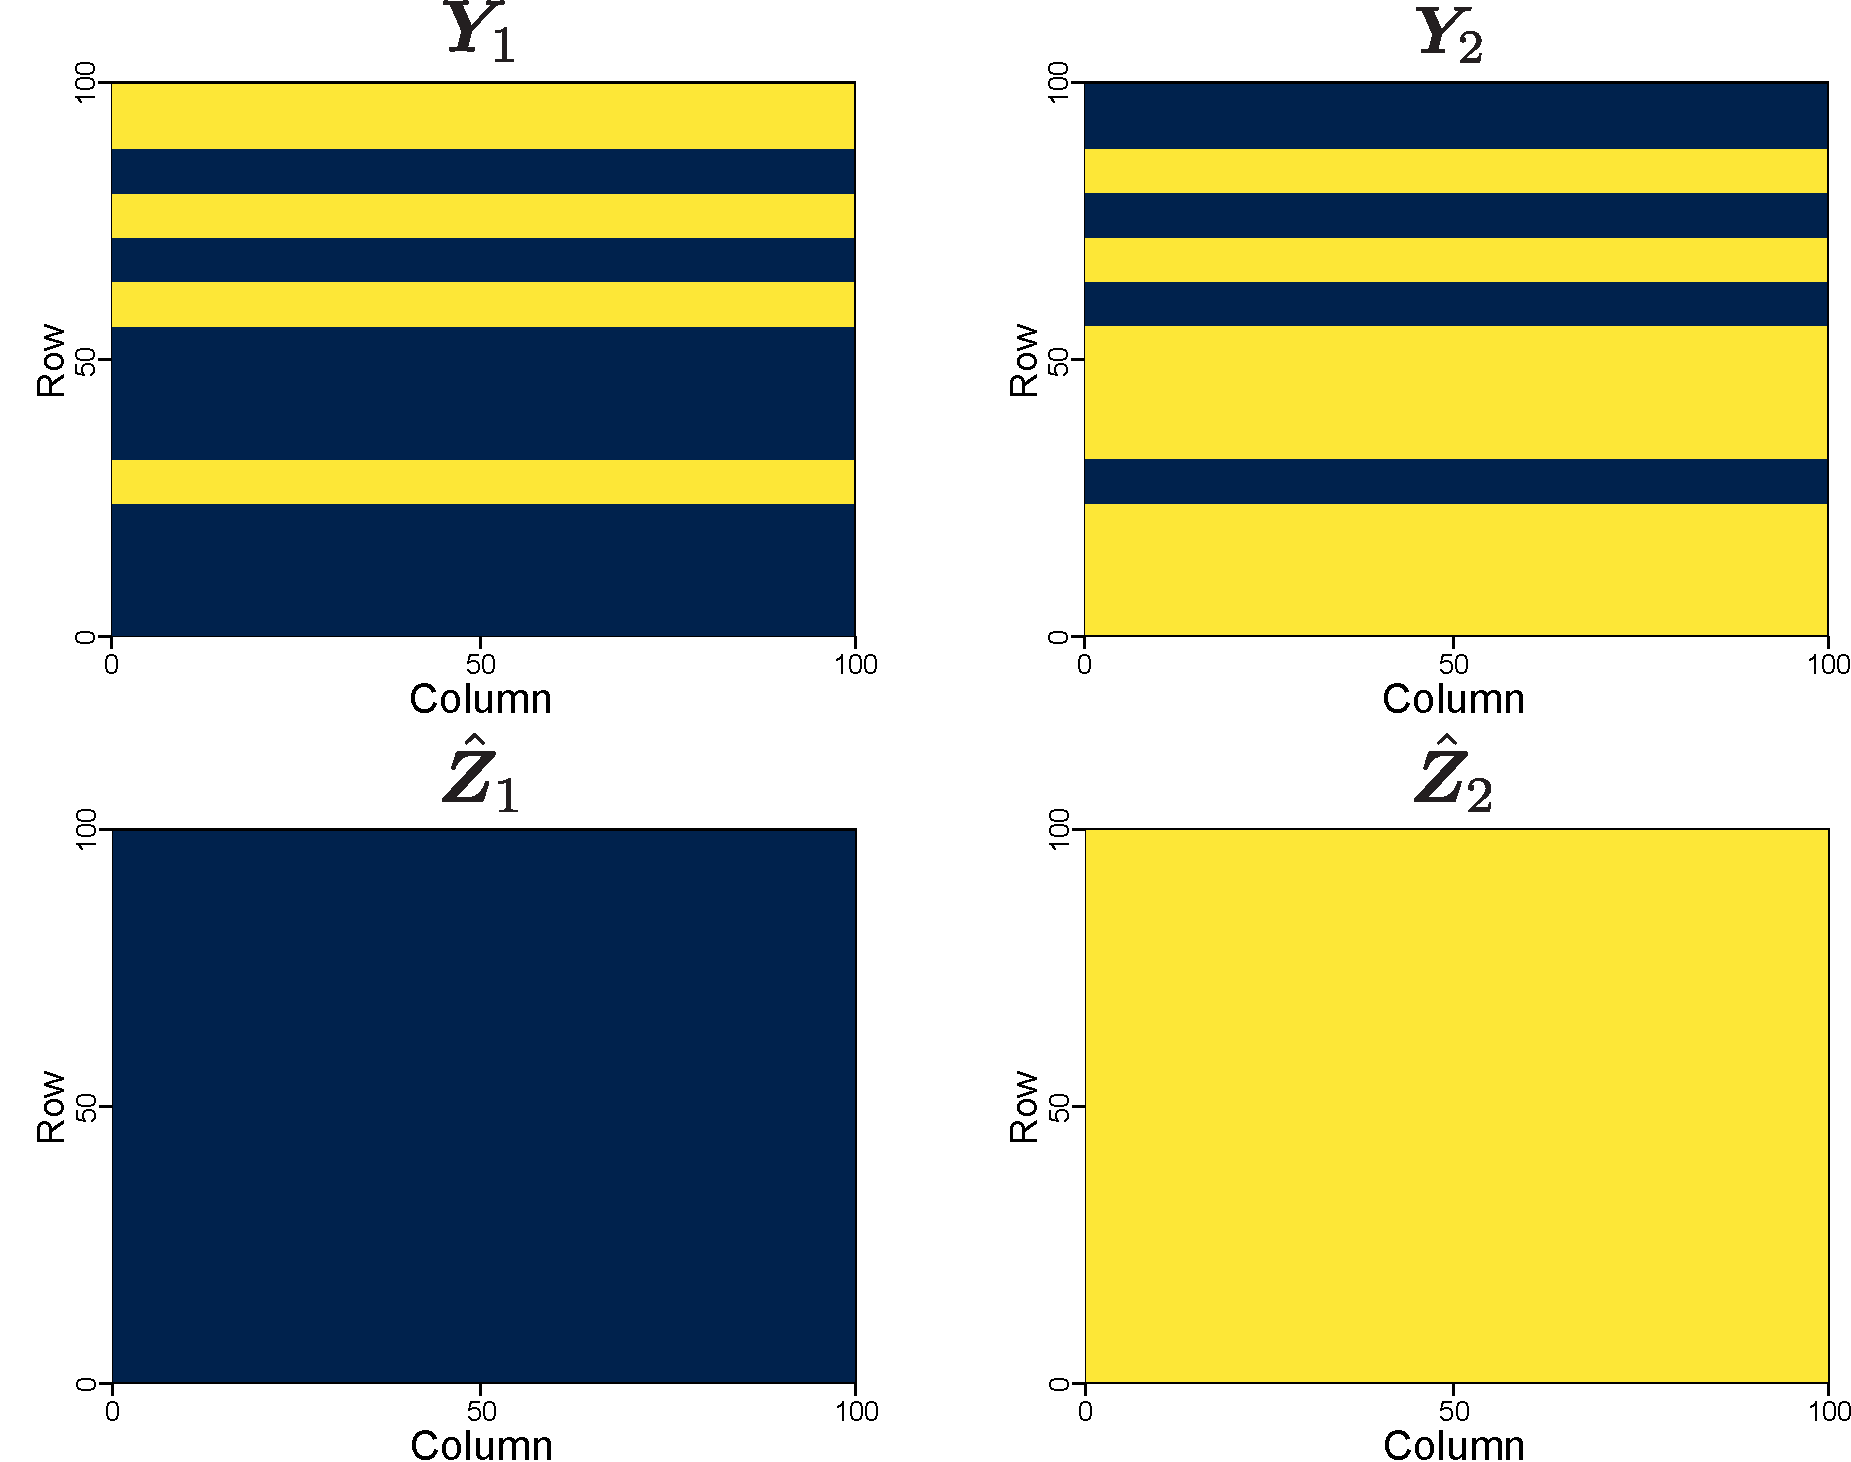
\includegraphics[clip, width=5.0in]{figures/01mat_8block.pdf}
    \label{fig:spec_01mat_8block}}  
    \caption{Experimental results using matrix of Fig~\ref{fig:01mat_spec} (randomly shuffle eight rows).}
    \label{fig:01mat_8block}
\end{figure*}
%%%%%%%%%%%%%%%%%%%%%%%%%%%%

%%%%%%%%%%%%%%%%%%%%%%%%%%%%
\begin{figure*}[!t]
    \centering
    \subfloat[Percentage of correct answers for training and validation data.]{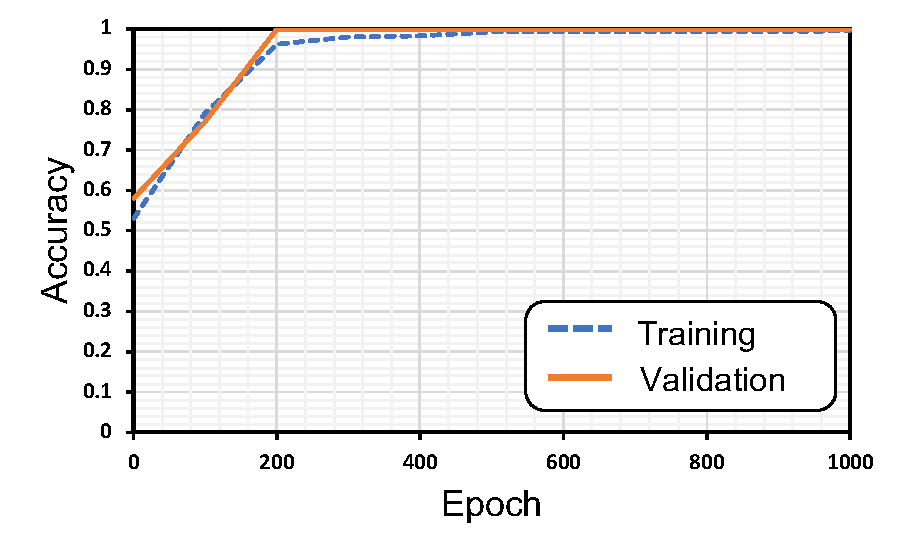
\includegraphics[clip, width=4.5in]{figures/graph/25stripe_8block.pdf}
    \label{fig:acc_25mat_8block}}
    \\
    \subfloat[Spectrogram of estimated signal and predictive separation signal.]{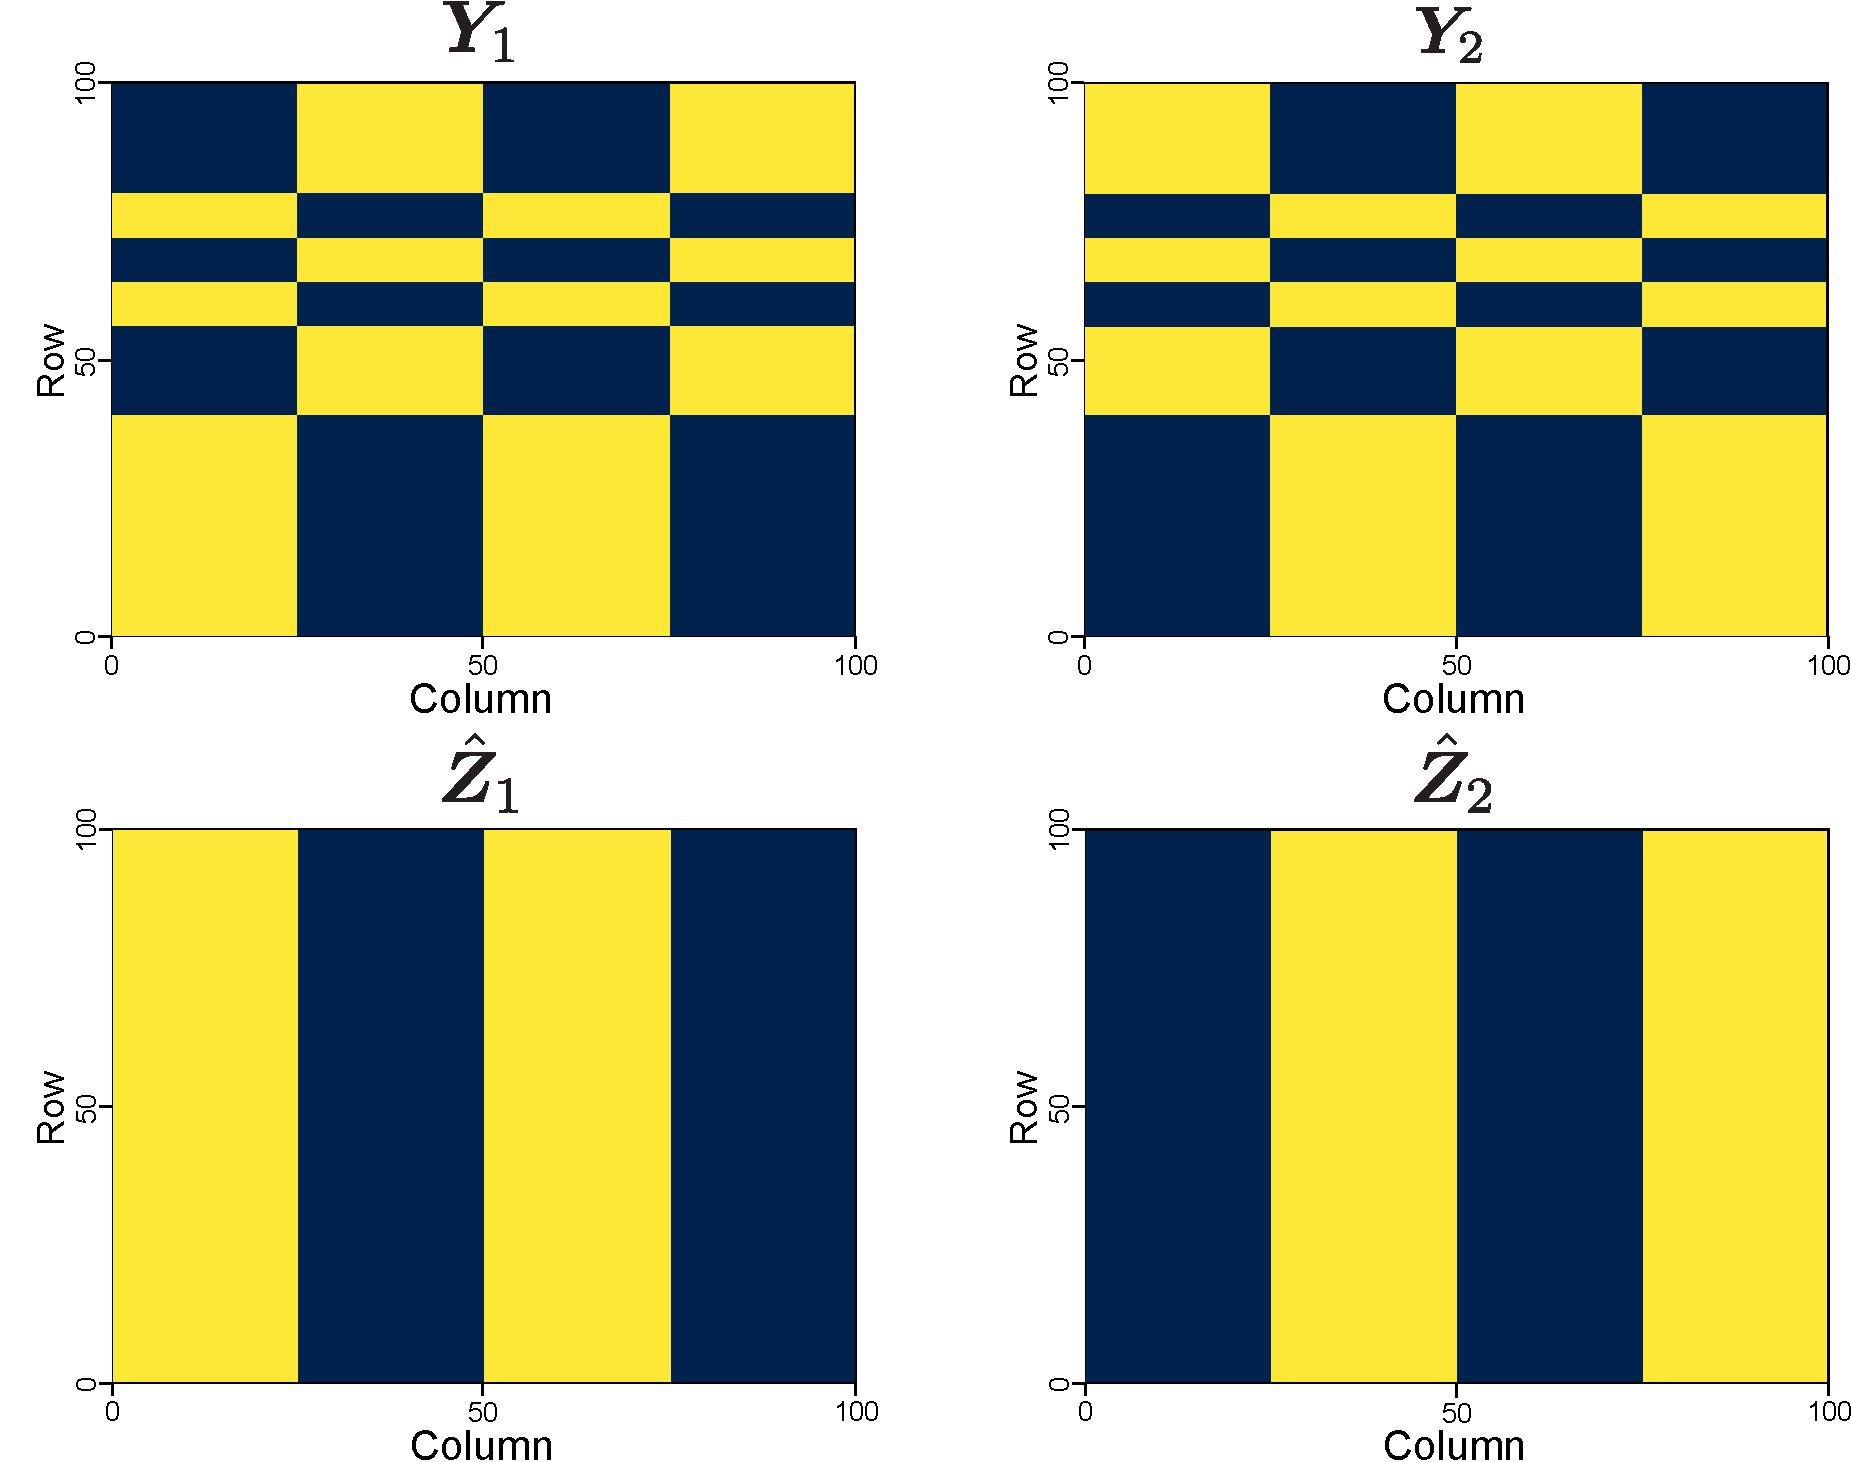
\includegraphics[clip, width=5.0in]{figures/25stripe_8block.pdf}
    \label{fig:spec_25mat_8block}}  
    \caption{Experimental results using the matrix of Fig~\ref{fig:25stripe_spec} (randomly shuffle eight rows).}
    \label{fig:25mat_8block}
\end{figure*}
%%%%%%%%%%%%%%%%%%%%%%%%%%%%

%%%%%%%%%%%%%%%%%%%%%%%%%%%%
\begin{figure*}[!t]
    \centering
    \subfloat[Percentage of correct answers for training and validation data.]{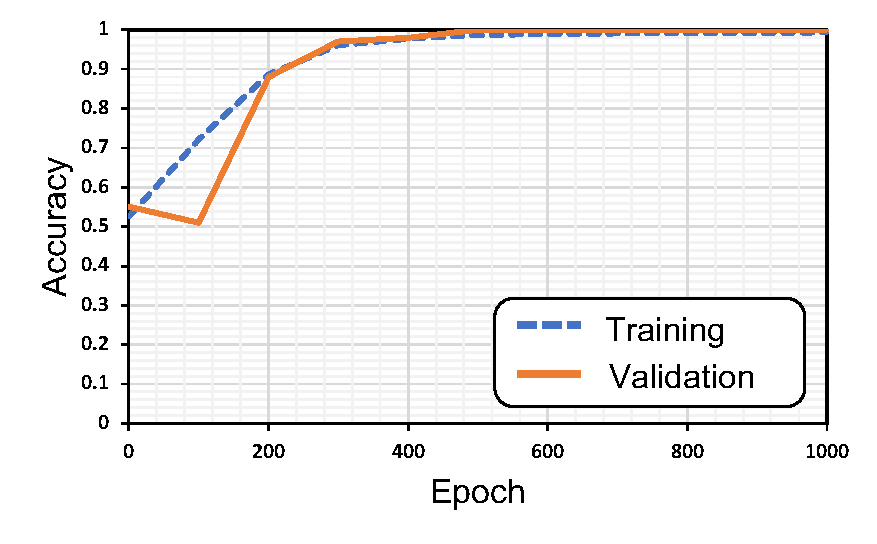
\includegraphics[clip, width=4.5in]{figures/graph/stripe_8block.pdf}
    \label{fig:acc_stripe_8block}}
    \\
    \subfloat[Spectrogram of estimated signal and predictive separation signal.]{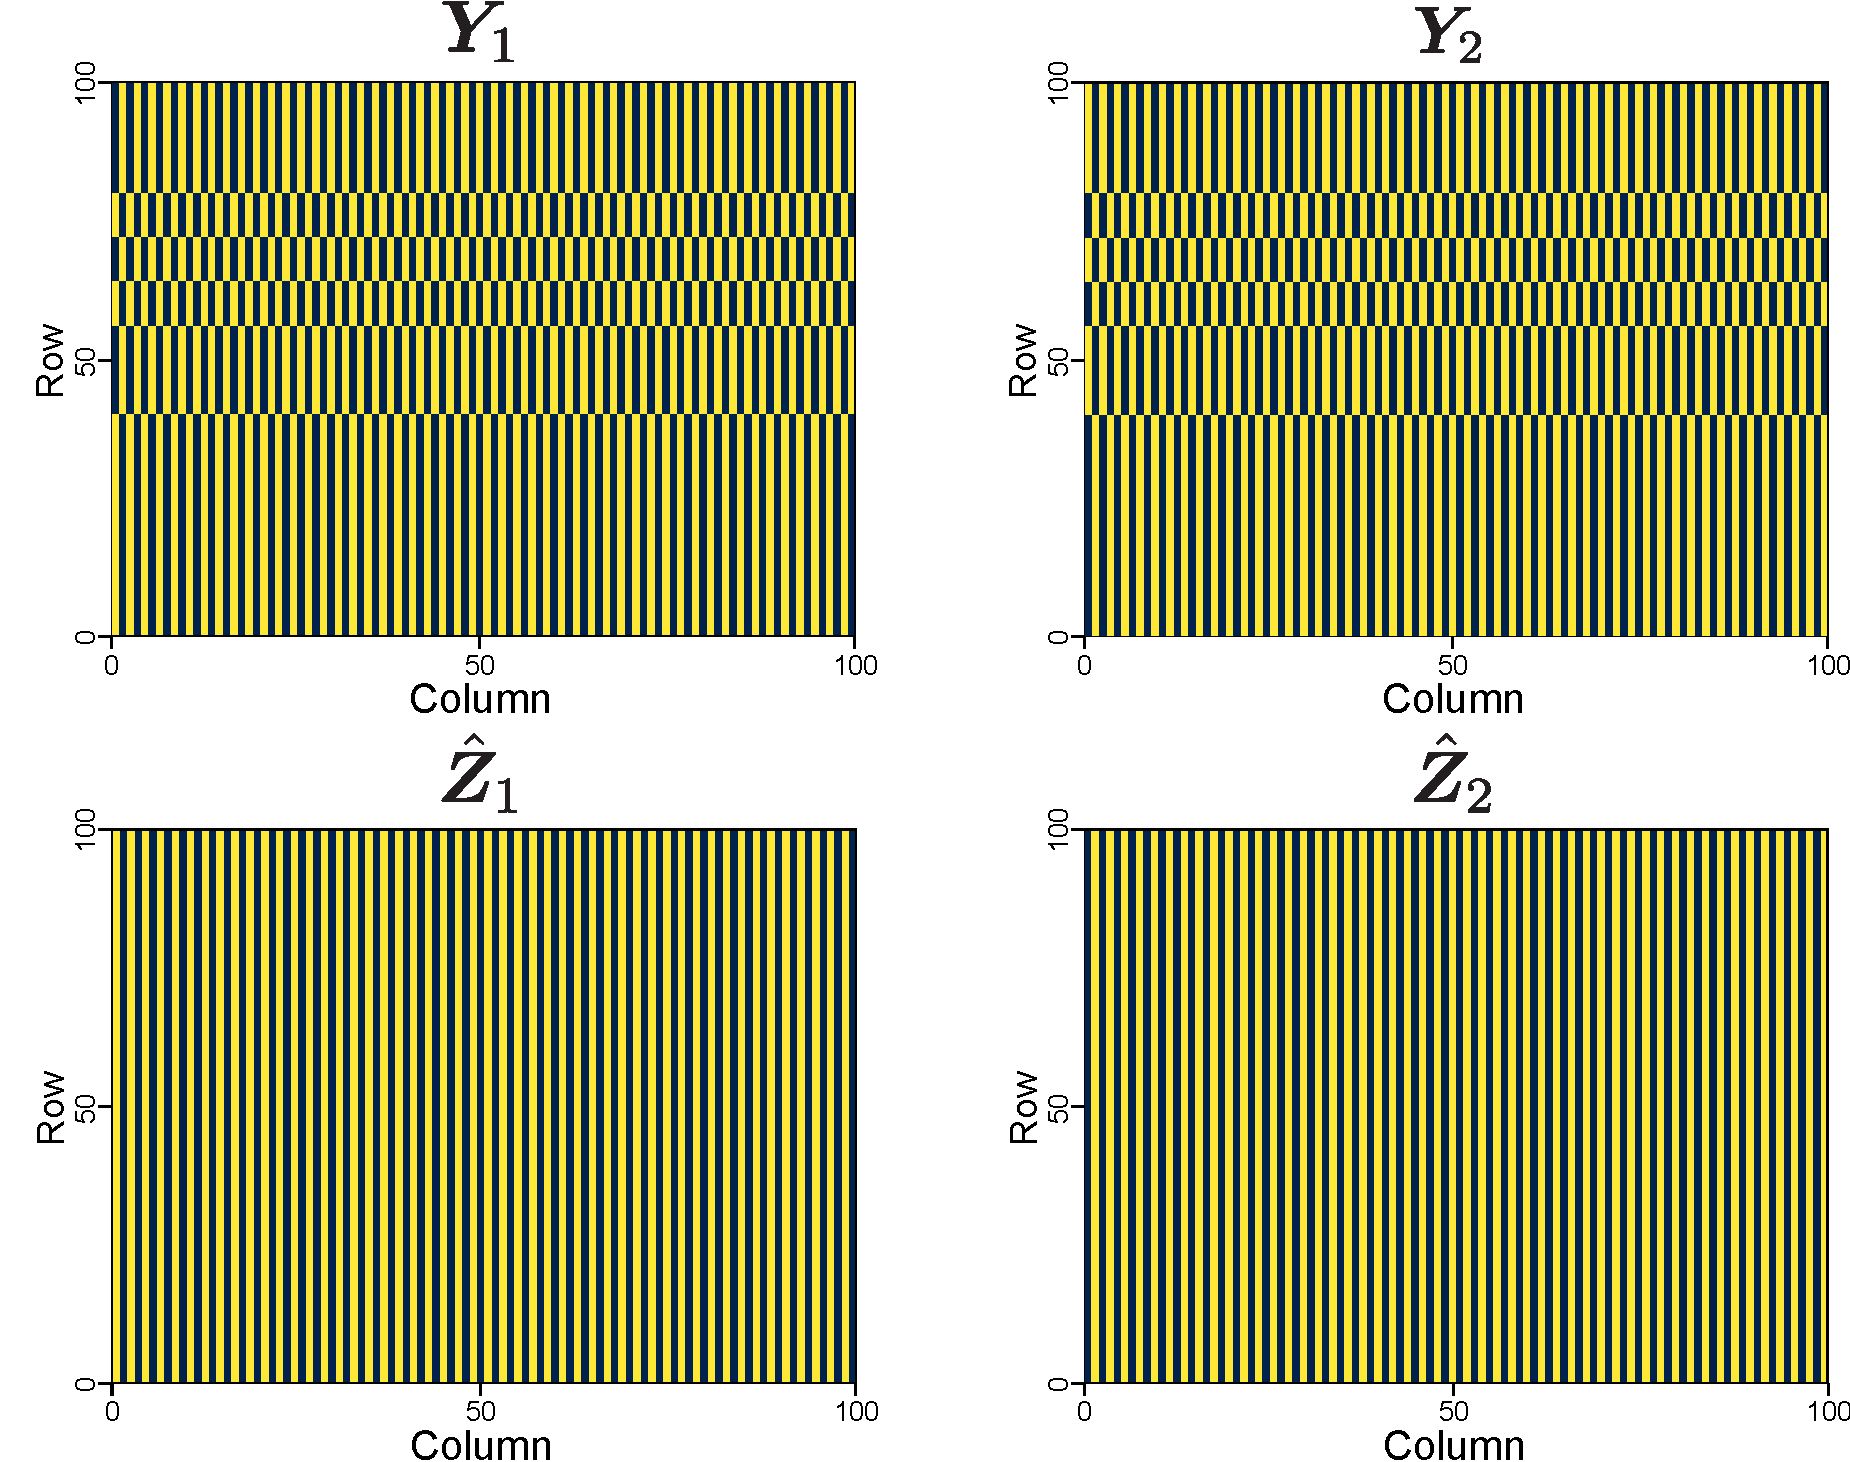
\includegraphics[clip, width=5.0in]{figures/stripe_8block.pdf}
    \label{fig:spec_stripe_8block}}  
    \caption{Experimental results using the matrix of Fig~\ref{fig:stripe_spec} (randomly shuffle eight rows).}
    \label{fig:stripe_8block}
\end{figure*}
%%%%%%%%%%%%%%%%%%%%%%%%%%%%
